\section{Verwendete Methoden Maschinellen Lernens}
\label{sec:lerner}
Zum Verständnis der Ergebnisse müssen zunächst die verwendeten
Lerner und Methoden erläutert werden, die zur Klassifikation
und Bewertung der Ergebnisse verwendet werden.

\subsection{Nächste-Nachbarn-Klassifikation}

Der k-Nächste-Nachbarn Klassifikator ist einer der einfachsten Lerner zur
Klassifikation. Die Klassen werden zugeordnet, in dem die $k$ nächsten Nachbarn
betrachtet werden. Dabei werden Abstandsmaße verwendet, wie beispielsweise
euklidische Abstände. Die Wahl des Parameters $k$ hat dabei einen hohen Einfluss
auf das Ergebniss, da ein zu geringer Wert hohe Sensitivität gegenüber Ausreißern
hat und ein zu hoher Wert, viele Einträge aus anderen Klassen beinhalten kann.
In Abbildung \ref{fig:knn} wird die Beeinflussung der Wahl der Anzahl der Nachbarn
verdeutlicht.

\begin{figure}
  \centering
  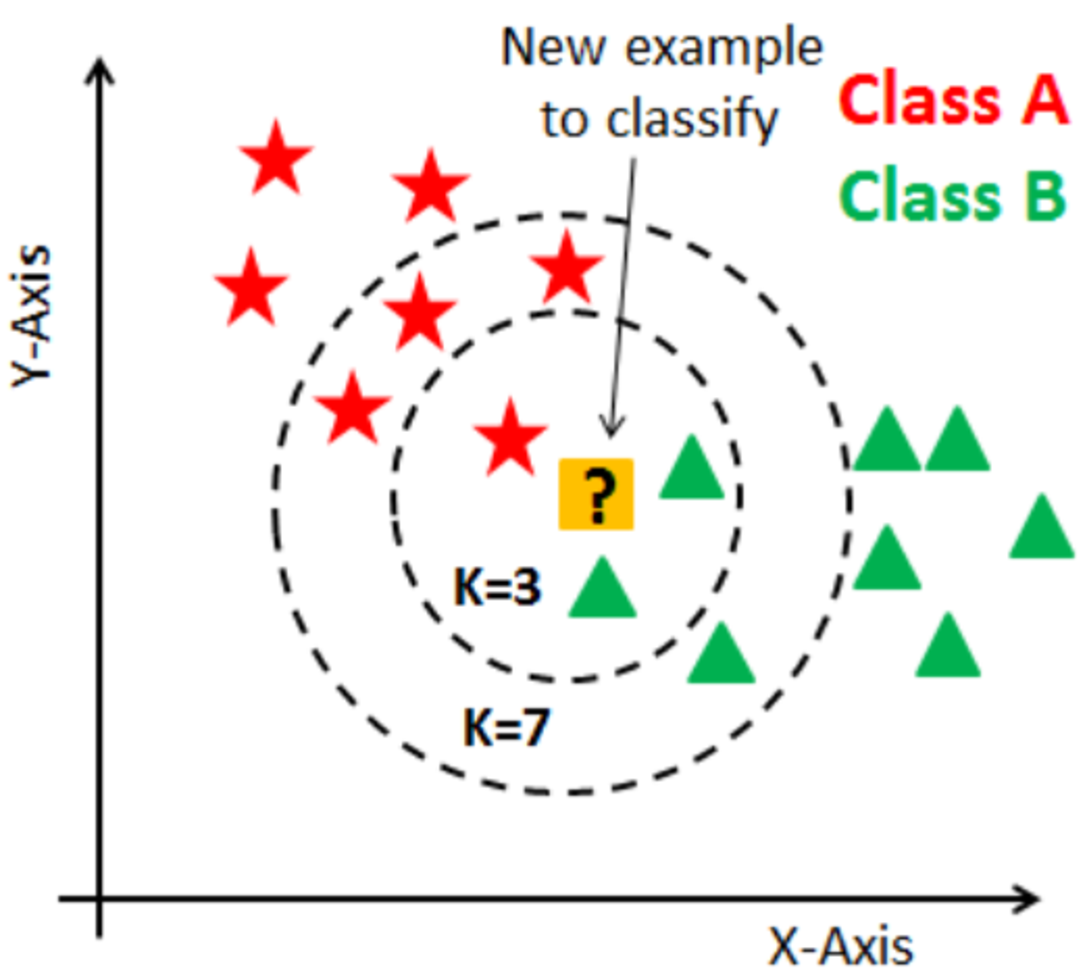
\includegraphics[width=0.5\textwidth]{plots/knn.pdf}
  \caption{Darstellung, wie die Wahl der Anzahl der Nachbarn die Klassifikation des Punktes
  beeinflussen kann. Bei $k = 3$ wird der Punkt Klasse B zugeordnet. Bei
  $k = 7$ wird der Punkt Klasse A zugeordnet \cite{kNN}.}
  \label{fig:knn}
\end{figure}

Ein
wichtiger Punkt des kNN-Lerners ist, dass er ein sogenannter \textit{lazy learner}
ist. Das bedeutet, beim Trainieren werden die Daten lediglich abgespeichert und
die Klassifikation findet nicht zeitgleich oder im Anschluss an das Training
statt, sondern erst, wenn die Klassifikation angefordert wird.


\subsection{Random Forest Klassifikationsverfahren}
Der \texttt{RandomForestClassifier} basiert auf binären Entscheidungsbäumen.
Bei einem Entscheidungsbaum wird an jedem Knoten ein Schnitt in einer Variable durchgeführt und die daraus entstandenen Teilmengen
werden in den beiden Ästen des Knotens wiederum durch Schnitte unterteilt, bis entweder eine bestimmte Tiefe
des Baumes erreicht ist oder die Blätter nur Ereignisse einer Klasse enthalten. Um die Effekte des Übertrainierens zu minimieren, wird über ein Ensemble unterschiedlicher
Entscheidungsbäume gemittelt.
Die Bäume werden dabei jeweils auf unterschiedlichen Teilmengen des Trainingsdatensatzes trainiert.
Die Attribute des Baumes an denen der beste Schnitt gesucht wird, werden zufällig ausgesucht.

\subsection{Naive-Bayes-Klassifikator}
Der Naive-Bayes Klassifikator beruht auf dem Satz von Bayes, der lautet:

\begin{equation*}
    p\left(A|B \right) = \frac{p\left(B|A \right) p\left(A \right)}{p\left(B \right)} \, .
\end{equation*}

Dabei kann $A$ der Klassenzugehörigkeit entsprechen, wobei gilt, dass
$A$ das Signal representiert und $\bar{A}$ den Untergrund. $B$ ist dann ein
Attribut. Der Klassifikator beruht auf der Annahme, dass die Attribute bedingt
unabhängig sind. Der Naive Bayes Lerner bestimmt die Wahrscheinlichkeit einer
Klasse durch Beobachtungen. Für das Beispiel der Attributswahl für
mehrere Attribute bei Signal und
Untergrund gilt, dass

\begin{equation*}
    Q = \prod\limits_{i = 1}^{n} \frac{p\left(B_i|A \right)}{p\left(B_i|\bar{A} \right)}
\end{equation*}
größer als Eins ist, wenn das Ereignis eher Signal als Untergrund entspricht.
Für $Q \textless 1$ gilt, dass das Ereignis wahrscheinlicher dem Untergrund
zugeordnet werden kann.

\subsection{Qualitätsparameter}
In der Analyse werden verschiedene Parameter verwendet um die Qualität der Klassifizierung
und die Stabilität der Attributsauswahl zu bewerten. Die dabei wichtigen Parameter
sind die Reinheit, die Effizienz und der Jaccard-Index. \par
Für die Berechnung der Reinheit und der Effizienz werden Werte benötigt, die
eine richtige oder falsche Einordnung identifizieren. Wird ein Ereignis dem
Parameter \textit{true positive $tp$} zugeordnet, bedeutet das beispielsweise,
dass die Zahl korrekt als Signal eingeordnet wurde. \textit{False positive $fp$}
bedeutet, die Zahl wurde als Signal eingeordnet, ist aber eigentlich ein
Untergrund. Als \textit{true negative $tn$} gilt eine Zahl, die richtig dem Untergrund
zugeordnet wurde und \textit{false negative $fn$} beschreibt ein Signal, welches
fälschlicherweise dem Untergrund zugeordnet wurde. Die Reinheit und die Effizienz
berechnen sich dann nach:

\begin{align*}
    \text{Reinheit}\, \, p &= \frac{tp}{tp + fp} \\
    \text{Effizienz}\, \, r &= \frac{tp}{tp + fn} \, .\\
\end{align*}

Der Jaccard-Index beschreibt die Stabilität der Attributsauswahl gegen statistische
Schwankungen im Lerner. Er wird berechnet über

\begin{equation*}
    J \left(F_a, F_b \right) = \frac{|F_a \cup F_b|}{|F_a \cap F_b|}
\end{equation*}
und beschreibt die Ähnlichkeit der beiden Mengen $F_a$ und $F_b$. Zur Bewertung
gilt dann:

\begin{equation*}
    \hat{J} = \frac{2}{l \left(l - 1 \right)} \sum\limits_{i = 1}^{l}\sum\limits_{j = i+1}^{l} J\left(F_i, F_j \right) \, .
\end{equation*}
Qualitativ bedeutet das, dass die Attributsauswahl $l$-mal auf $l$ Teilmengen des Datensatzes durchgeführt wird. Der Index
selber dient dazu, die Ähnlichkeit der verschiedenen Selektionen zu beurteilen. Ist der Index nahe eins, ist die
Attributsauswahl stabil gegenüber statistischen Schankungen.

\subsection{Kreuzvalidierung}

Kreuzvalidierung wird benötigt, um einen Fehler auf die Qualitätsparameter der Reinheit und der Efiizienz angeben zu
können. Diese Fehler entstehen dann durch statistische Schwankungen im Trainingsdatensatz. Dieser wird in $n$ Teile
aufgeteilt und der Lerner dann auf $n-1$ Teile trainiert. Das dadurch erstellte Modell wird zur Klassifizierung des
übrigen Teils des Trainingsdatensatzes getestet. Diese Methode wird $n$ mal wiederholt, sodass jeder Teil der $n$
Teile des Trainingsdatensatz einmal als Testdatensatz verwendet wird. Somit werden im Endeffekt $n$ Werte für die
Effizienz und Reinheit ermittelt, von denen dann der Mittelwert und die Standardabweichung berechnet werden können.

\subsection{ROC-Kurven}

In einer ROC-Kurve\footnote{receiver operated characteristic} wird die relative Häufigkeit der \textit{true positives} an der 
die relative Häufigkeit der
\textit{false positives} aufgetragen. Eine Grade, die zwischen den Punkten
$\left(0,0 \right)$ und $\left(1,1 \right)$ verläuft, stellt ein Modell
des puren Zufalls da, da für jeden möglichen Wert auf dem Modell immer gleich viele
richtig und falsch positive Fälle vorhanden sind. Es ist somit wünschenswert, dass
sich die getesten Modelle immer oberhalb dieser Kurve und möglichst nah am linken
äußeren Rand befinden. Denn dort ist die \textit{true positives} Rate, also
die relative Häufigkeit der korrekt als richtig eingeordneten Ereignisse maximal
und die \textit{false positives} Rate, also die falsch eingeordneten Ereignisse
der Kategorie "positiv" maximal. \par
Als ROC AUC wird die \textit{Area unter the curve} bezeichnet, also die Fläche
unterhalb der ROC-Kurve. Im Fall der Graden zwischen den Punkten $\left(0,0 \right)$ und $\left(1,1 \right)$
wäre der ROC-AUC-Score $0.5$. Modelle, die nah an $0.5$ liegen, sind somit
schlecht konditioniert und spiegeln den reinen Zufall wieder, wohingegen
Modelle mit einem ROC-AUC-Score nahe der $1$ ein gutes Modell widerspiegeln.
